% ResearchIQ manuscript — restructured for "Information Technologies and Learning Tools" (ITLT)
% Ukrainian, ITLT structure (Introduction / Theoretical backgrounds + Methods / Findings / Conclusions).
% Tectonic-friendly preamble; body kept pandoc-convertible (no tikz; booktabs tables; \includegraphics).
\documentclass[12pt,a4paper]{article}
\usepackage{fontspec}
\usepackage{polyglossia}
\setmainlanguage{ukrainian}
\setotherlanguage{english}
\setmainfont{DejaVu Serif}
\setsansfont{DejaVu Sans}
\setmonofont{DejaVu Sans Mono}
\usepackage{geometry}
\geometry{margin=2.5cm}        % ITLT: all margins 2.5 cm
\usepackage{setspace}
\singlespacing                  % ITLT: single spacing
\usepackage{booktabs,longtable,array}
\usepackage{amsmath,amssymb}
\usepackage{graphicx}
\graphicspath{{../figures/}}
\usepackage[numbers,sort&compress]{natbib}
\usepackage{hyperref}
\hypersetup{hidelinks}
\setlength{\parindent}{1em}     % ITLT: first-line indent

\begin{document}

% ---- Front matter (ITLT) ----
\noindent УДК 004.9:001.89:378 \hfill % [UNCONFIRMED — confirm UDC with editor]

\begin{center}
{\large\bfseries ГЕНЕРАТИВНИЙ ШТУЧНИЙ ІНТЕЛЕКТ ТА АВТОНОМНІ АГЕНТИ В УПРАВЛІННІ НАУКОВОЮ ДІЯЛЬНІСТЮ ЗАКЛАДІВ ВИЩОЇ ОСВІТИ: КОНЦЕПТУАЛЬНА МОДЕЛЬ І ВІДТВОРЮВАНА АПРОБАЦІЯ}
\end{center}

\vspace{0.5em}
\noindent\textbf{Заболотній Сергій Васильович}\\
доктор технічних наук, професор\\
Черкаський державний бізнес-коледж, м.~Черкаси, Україна\\
\textit{ORCID: 0000-0000-0000-0000} % [UNCONFIRMED — insert author ORCID]\\
\textit{zabolotniisv@... } % [UNCONFIRMED — insert email]

\vspace{1em}

% ---- Abstracts (UA + EN) + keywords ----
\textbf{Анотація.} Цифрова трансформація наукового адміністрування закладів вищої освіти стримується фрагментацією наукометричних даних між ORCID, Scopus, Web of Science та OpenAlex. Неузгодженість ідентифікаторів, транслітерацій і метаданих призводить до 15--25\,\% дублікатів у типових звітах, а підготовка звітності потребує значної ручної верифікації. Мета статті --- обґрунтувати модель і механізми інтеграції GenAI та автономних агентів для проактивного управління науковою діяльністю ЗВО засобами ІКТ. Запропоновано ResearchIQ --- багатокористувацький вебзастосунок із React-інтерфейсом, Node.js API, tenant-сховищем даних і агентним шаром на основі \texttt{pi-agent-core}. Агент отримує локальний знімок даних ЗВО, викликає типізовані інструменти пошуку, ранжування, порівняння кафедр, побудови профілів, глобального пошуку праць і формування звітів, але не ухвалює критичних рішень щодо тотожності публікацій. Ядром обробки є «золотий запис» (Golden Record) --- конвеєр розв'язання сутностей із канонізацією метаданих, блокуванням, парним логістичним зіставленням, кластеризацією, провенансом і смугою перевірки людиною. Архітектуру спроєктовано за рамкою TRACE: детерміноване ядро, класичне машинне навчання та мовну модель-валідатор рознесено в окремі шари, а ощадливе використання LLM для структурованих даних виражено коефіцієнтом обчислювальної ощадливості. Модель апробовано на відтворюваному синтетичному бенчмарку, що імітує реалістичний український ЗВО (300 науково-педагогічних працівників, 20 кафедр, близько 5 факультетів) без персональних даних; статистичну стійкість оцінено методом Монте-Карло (K=30). Кількісну апробацію зосереджено на детермінованому ядрі дедуплікації; агентний шар подано як концептуальний природномовний інтерфейс, що не бере участі в обчисленні метрик. Golden Record досяг F1 76,8\,\% проти 59,7\,\% для DOI-only та 53,5\,\% для Title+Year. Виправлено дефект нормалізатора, що знищував 100\,\% україномовних назв публікацій. Аналітична модель оцінює ручну працю в 429,1 год/рік на ЗВО проти 2,11 с машинного обчислення. Результати позиціонують підхід як реалістичну стратегію цифрової трансформації наукового адміністрування.

\textbf{Ключові слова:} ІКТ в управлінні освітою; цифрова трансформація наукового адміністрування; генеративний штучний інтелект; автономний агент (MCP); золотий запис і розв'язання сутностей; проактивне управління науковою діяльністю ЗВО.

\bigskip

\textbf{Abstract.} The digital transformation of research administration in higher education institutions is hindered by fragmented scientometric data distributed across ORCID, Scopus, Web of Science, and OpenAlex. Inconsistent identifiers, transliterations, and metadata cause 15--25\,\% of records in typical reports to be duplicates and require substantial manual verification. The aim of the article is to substantiate a model and integration mechanisms for GenAI and autonomous agents that support proactive HEI research management through ICT. We propose ResearchIQ, a multi-tenant web application with a React interface, a Node.js API, tenant data storage, and an agent layer based on \texttt{pi-agent-core}. The agent receives a local HEI data snapshot and invokes typed tools for search, ranking, department comparison, faculty profiles, global work search, and report generation, but it does not make critical publication-identity decisions. The data-processing core is the Golden Record --- an Entity Resolution pipeline with metadata canonicalisation, blocking, pairwise logistic matching, clustering, provenance tracking, and a human-in-the-loop review band. The architecture follows the TRACE framework: a deterministic core, classical machine learning, and an LLM validator are separated into distinct layers, and parsimonious LLM use for structured-data tasks is expressed by the Computational Parsimony Ratio. The model is evaluated on a reproducible synthetic benchmark simulating a realistic Ukrainian HEI (300 academic staff, 20 departments, about 5 faculties) without personal data; statistical robustness is assessed by Monte Carlo simulation (K=30). The quantitative evaluation targets the deterministic deduplication core; the agent layer is a conceptual natural-language interface and is not itself benchmarked here. The Golden Record pipeline achieves an F1 score of 76.8\,\% versus 59.7\,\% for DOI-only and 53.5\,\% for Title+Year. A critical normaliser defect that destroyed 100\,\% of Ukrainian-language publication titles was corrected. An analytical efficiency model estimates manual effort at 429.1 hours per HEI-year compared with 2.11 seconds of machine computation. The findings position the approach as a realistic ICT strategy for transforming HEI research administration.

\textbf{Keywords:} ICT in education management; digital transformation of research administration; generative artificial intelligence; autonomous agent (MCP); Golden Record and Entity Resolution; proactive management of HEI research activity.


% ---- Body ----
\section*{ВСТУП}

\subsection*{Постановка проблеми}

Цифрова трансформація системи вищої освіти України дедалі більше зміщується із площини організації навчального процесу у площину управління науковою діяльністю закладів вищої освіти (ЗВО). Інтеграція до європейського дослідницького простору, вимоги відкритої науки та потреба об'єктивної оцінки наукової результативності перетворюють інформаційно-комунікаційні технології (ІКТ) наукового адміністрування на критичну інфраструктуру управління освітою. Водночас обсяги наукової інформації, з якими має оперувати адміністрація ЗВО, зростають швидше за можливості традиційних, переважно ручних, процедур обліку. За даними відкритої наукометричної бази OpenAlex, світовий масив наукових праць перевищив 250 млн записів і поповнюється приблизно на 5 млн праць щороку \cite{OpenAlex2024Docs}. У таких умовах реактивна модель бібліометричної звітності, за якої заклад фіксує результати \textit{post factum} --- наприкінці звітного періоду, --- вичерпує себе й перетворюється на джерело управлінських ризиків.

Аналіз практики наукового адміністрування ЗВО дає змогу виокремити чотири взаємопов'язані проблеми, що утворюють ядро суперечності між наявними та потрібними механізмами цифрового управління наукою.

\textit{По-перше, фрагментація даних про наукову продуктивність.} Відомості про публікації одного й того самого науковця розосереджені між профілями ORCID, реферативними базами Scopus і Web of Science та відкритою базою OpenAlex. Ці джерела використовують несумісні ідентифікатори, по-різному транслітерують прізвища (наприклад, \textit{Заболотній С.} та \textit{Zabolotnii S.}), скорочують назви видань і подають метадані з різною повнотою. Унаслідок цього в типових кафедральних та факультетських звітах від 15\,\% до 25\,\% записів виявляються дублікатами однієї канонічної праці. Без коректного зведення сутностей будь-який агрегований показник --- кількість публікацій, сумарна цитованість, частка відкритого доступу --- системно спотворюється.

\textit{По-друге, надмірна трудомісткість підготовки звітності.} Формування річного звіту кафедри включає копіювання записів із кількох систем, звіряння варіантів однієї праці, усунення дублікатів і форматування переліків відповідно до вимог Міністерства освіти і науки України щодо фахових видань \cite{MONUkraine2023ProfessionalJournalsOrder}. У зовнішніх дослідженнях адміністративного навантаження науковців звітні й супровідні процедури також фіксуються як суттєва частка дослідницького часу: у FDP Faculty Burden Survey 6081 PI/Co-PI повідомили, що в середньому 42\,\% часу, відведеного на federally funded research, витрачається на адміністративні задачі, серед яких подання звітів про прогрес грантів входить до найвідчутніших навантажень \cite{Rockwell2009FDPBurden}. Тому інтервал 8--12 год для малої або середньої кафедри використано в цій роботі не як універсальний емпіричний норматив, а як консервативний калібрувальний орієнтир для подальшої прозорої моделі ручної праці. Така праця є рутинною, погано масштабованою та схильною до помилок, а її обсяг зростає з кількістю науково-педагогічних працівників і публікацій.

\textit{По-третє, реактивність моделі управління.} Чинні інформаційні процедури фіксують уже здобуті результати, але не підтримують випереджального аналізу: керівництво ЗВО не отримує своєчасних сигналів про відставання окремих підрозділів, про публікації в журналах із сумнівною репутацією чи про незадеклароване співавторство. Управлінські рішення приймаються із запізненням на цілий звітний цикл.

\textit{По-четверте, відсутність науково обґрунтованих механізмів інтеграції генеративного штучного інтелекту (GenAI) у наукове адміністрування.} Попри стрімке поширення великих мовних моделей, концептуальні моделі та відтворювані механізми їх застосування саме до завдань управління науковою діяльністю ЗВО фактично не розроблені, а наявні поодинокі рішення мають характер непрозорих евристик без верифікованої якості.

Сукупність цих проблем зумовлює \textit{актуальність} розроблення концептуальної моделі та технологічних механізмів переходу від реактивної бібліометричної звітності до проактивного управління науковою діяльністю ЗВО засобами ІКТ. Розв'язання цього завдання має водночас управлінсько-освітній та технологічний вимір, що й визначає його належність до проблематики ІКТ в управлінні освітою.

\subsection*{Аналіз останніх досліджень і публікацій}

Застосування генеративного ШІ у вищій освіті є предметом інтенсивних досліджень, проте їх тематичний фокус виявляє суттєву прогалину. Систематичний огляд Т.~Тіллманнса та співавторів показує переважання дидактичних сценаріїв GenAI у вищій освіті \cite{Tillmanns2025SystematicReviewGenAIHE}; емпіричне дослідження А.~Альшамі та співавторів деталізує сприйняття таких інструментів студентами й академічним персоналом \cite{Alshamy2025PerceptionsGenAIHE}. Натомість \textit{адміністративна} сфера, зокрема управління науковою діяльністю та наукова звітність ЗВО, лишається майже поза увагою. Саме ця незаповнена ніша визначає простір новизни нашого дослідження: ми переносимо інструментарій GenAI з дидактичної площини у площину цифрового управління наукою.

Концептуальним підґрунтям такого перенесення слугує сфера управління дослідницькою інформацією (Research Information Management, RIM) та системи поточної дослідницької інформації (Current Research Information Systems, CRIS) \cite{Bryant2017RIMDefining}. Розвиток цих систем у Європі координується ініціативами OpenAIRE та Європейською хмарою відкритої науки (EOSC), які формують вимоги до сумісності й якості дослідницьких даних \cite{OpenAIRE2023GuidelinesCRIS}, а семантичну сумісність метаданих про наукову діяльність забезпечує стандарт CERIF \cite{euroCRIS2024CERIF}. Для українських ЗВО опанування цього інструментарію є складовою євроінтеграції наукової сфери. Проте класичні CRIS зорієнтовані переважно на пасивне зберігання та обмін даними й не передбачають автономного, інтелектуального опрацювання фрагментованих джерел --- саме тут відкривається можливість для якісно нового рівня автоматизації.

Технологічною передумовою такого рівня стала поява механізмів керованої взаємодії мовних моделей із зовнішніми інструментами та даними. Протокол Model Context Protocol (MCP), оприлюднений компанією Anthropic у листопаді 2024 р. \cite{Anthropic2024MCP}, стандартизує підключення автономних агентів до зовнішніх джерел через виклик функцій (Function Calling) і дає змогу будувати агентів, здатних не лише генерувати текст, а й виконувати верифіковані операції над даними наукових профілів. Це перетворює GenAI з генератора відповідей на компонент керованого обчислювального конвеєра.

Водночас застосування мовних моделей в управлінні, де ціна помилки висока, наражається на принциповий ризик --- генерування правдоподібних, але хибних тверджень (галюцинацій). Емпіричні дослідження фіксують відчутну частоту таких помилок навіть у спеціалізованих задачах опрацювання наукової літератури \cite{Chelli2024HallucinationRates}. Звідси випливає методологічна вимога: відповідальні управлінські рішення (зокрема об'єднання записів про публікації) не можна повністю делегувати мовній моделі. Детерміновані, перевірювані процедури мають відповідати за критичні операції, а людина-експерт --- залишатися в контурі прийняття рішень (human-in-the-loop, HITL) у зонах невизначеності.

Завдання усунення дублікатів і зведення розрізнених записів до єдиної канонічної сутності є окремим випадком класичної проблеми розв'язання сутностей (Entity Resolution, ER). Її розв'язком у нашій моделі є побудова «золотого запису» (Golden Record) --- консолідованого, очищеного від дублікатів і збагаченого провенансом подання кожної праці. Як методологічну рамку для проєктування й оцінювання відповідного програмного артефакту обрано методологію проєктування на основі дизайн-науки (Design Science Research, DSR): класична праця А.~Хевнера та співавторів задає вимогу створення корисного артефакту \cite{Hevner2004DSR}, К.~Пефферс та співавтори формалізують процес DSR-оцінювання \cite{Peffers2007DSRMeth}, а Ш.~Грегор і А.~Хевнер уточнюють спосіб позиціонування внеску \cite{Gregor2013PositioningDSR}. DSR забезпечує наукову обґрунтованість запропонованих механізмів і відтворюваність їх апробації.

Отже, на перетині трьох напрямів --- перенесення GenAI з навчання в адміністрування науки, інтеграції автономних агентів через MCP у системи RIM/CRIS та контрольованого людиною розв'язання сутностей --- утворюється недостатньо досліджена проблемна область, опрацювання якої й становить мету цієї статті.

\subsection*{Мета і завдання статті}

\textbf{Мета статті} --- розробити та апробувати концептуальну модель і технологічні механізми інтеграції генеративного ШІ та автономних агентів для переходу від реактивної бібліометричної звітності до проактивного управління науковою діяльністю ЗВО засобами ІКТ, спроєктувавши їх на засадах інженерної рамки TRACE для побудови довірених агентних систем у сферах із високою ціною помилки \cite{Zabolotnii2026TRACE}.

Досягнення поставленої мети передбачає розв'язання таких завдань:

\begin{enumerate}
    \item обґрунтувати концептуальну модель проактивного управління науковою діяльністю ЗВО, що інтегрує GenAI та автономних агентів (MCP) у контур наукового адміністрування й узгоджується з підходами RIM/CRIS та стандартом CERIF;
    \item спроєктувати архітектуру системи за інженерною рамкою TRACE, рознісши компоненти на детерміноване ядро (L1), класичний ML (L2a), мовну модель-валідатор (L2b) та політику ескалації з наглядом людини (L3/L4), і обґрунтувати ощадливе застосування LLM за принципом ощадливості моделі (Model Parsimony) із кількісним індикатором --- коефіцієнтом обчислювальної ощадливості (CPR);
    \item формалізувати конвеєр розв'язання сутностей для побудови «золотого запису» над джерелами ORCID, OpenAlex і Scopus, зокрема процедури канонізації метаданих із коректним опрацюванням кириличних назв, блокування, парного зіставлення та кластеризації із захистом від хибних злиттів;
    \item визначити роль людини в контурі (HITL) як механізм пом'якшення ризику галюцинацій GenAI шляхом винесення невизначених випадків зіставлення на ручну перевірку;
    \item розробити відтворюваний синтетичний бенчмарк на узагальненому модельному середньому українському ЗВО для оцінювання якості дедуплікації та злиття записів без використання персональних даних;
    \item експериментально оцінити ефективність запропонованих механізмів за метриками якості (Precision, Recall, F1, B\textsuperscript{3} F1) у порівнянні з базовими підходами та проаналізувати чутливість результатів до частки дублікатів і ступеня спотворення метаданих;
    \item на основі прозорої аналітичної моделі оцінити потенціал скорочення трудомісткості наукової звітності та окреслити обмеження й загрози валідності запропонованого підходу.
\end{enumerate}

\section*{ТЕОРЕТИЧНІ ОСНОВИ ТА МЕТОДИ ДОСЛІДЖЕННЯ}

Методологічним підґрунтям дослідження є парадигма науки про проєктування (Design Science Research, DSR), яка зорієнтована на створення та оцінювання артефактів, що розв'язують практично значущі проблеми управління \cite{Hevner2004DSR}. Процедурну логіку побудови й оцінювання артефакту уточнено за методологією К.~Пефферса та співавторів \cite{Peffers2007DSRMeth}. У межах цієї парадигми артефактом виступає концептуальна модель і реалізований програмний механізм інтеграції генеративного штучного інтелекту (GenAI) та автономних агентів у процеси наукового адміністрування (research information management, RIM) закладу вищої освіти (ЗВО). Виклад побудовано як послідовність: концептуальна рамка переходу від реактивної до проактивної моделі управління $\rightarrow$ архітектура інтеграції GenAI $\rightarrow$ ядро механізму (золотий запис як конвеєр розв'язання сутностей) $\rightarrow$ дизайн відтворюваного оцінювання.

\subsection*{Реактивна та проактивна моделі управління науковою діяльністю}

Цифрова трансформація публічного та університетського управління — це не автоматизація наявних паперових процедур, а перепроєктування самих управлінських практик навколо даних \cite{Mergel2019DefiningDigitalTransformation}. Концепція цифрового врядування (digital-era governance) наголошує на реінтеграції розрізнених інформаційних потоків, переході до потребо-орієнтованої цілісності та цифровізації як організаційного, а не лише технічного зрушення \cite{Dunleavy2006DigitalEraGovernance}. Управління науковою інформацією (RIM) як окрема функція ЗВО систематизує дані про публікації, проєкти, авторів та результати для підтримки ухвалення рішень \cite{Bryant2017RIMDefining}.

Реактивна бібліометрична звітність працює за принципом \emph{post factum}: дані збирають уручну після завершення звітного періоду, верифікують і форматують під вимоги регулятора. Така модель має три системні вади. По-перше, висока трудомісткість: навіть консервативний сценарій малої або середньої кафедри передбачає кілька годин копіювання, звіряння та форматування, а опубліковані дослідження адміністративного навантаження науковців підтверджують, що звітні процедури є значною частиною дослідницького workflow \cite{Rockwell2009FDPBurden}. По-друге, фрагментація даних між незалежними джерелами (ORCID, Scopus, Web of Science, OpenAlex) породжує 15--25\,\% дублікатів у типових звітах. По-третє, реактивність позбавляє керівництво кафедри чи факультету можливості раннього втручання — рішення ухвалюють тоді, коли результат уже зафіксовано.

Проактивна модель управління науковою діяльністю натомість трактує наукометричні дані як безперервний керований потік. Інтегрований «золотий запис» дослідника й підрозділу оновлюється інкрементно, а керівник отримує доступ до актуальної картини в будь-який момент, а не лише наприкінці року. Це узгоджується з логікою євроінтеграції українського наукового простору: інфраструктури OpenAIRE та EOSC вимагають машиночитаних, інтероперабельних і безперервно підтримуваних даних \cite{OpenAIRE2023GuidelinesCRIS}, а модель RIM/CRIS описує організаційну роль таких даних у дослідницькому управлінні \cite{Bryant2017RIMDefining}. Стандарт CERIF, своєю чергою, задає канонічну схему сутностей наукової діяльності \cite{euroCRIS2024CERIF}. Перехід до проактивності — це передусім управлінське, а вже потім технічне завдання: змінюється не інструмент звітування, а сам цикл прийняття рішень.

\subsection*{Інженерна рамка TRACE: пошарова організація та ощадливість моделі}

Описане розмежування ролей систематизовано за інженерною рамкою \emph{TRACE}, призначеною для побудови довірених агентних систем у сферах з високою ціною помилки \cite{Zabolotnii2026TRACE}. Її засаднича теза --- довіра є властивістю \emph{архітектури}, а не окремої моделі, --- безпосередньо відповідає вимогам відповідального адміністрування. У термінах TRACE компоненти запропонованої системи розподіляються на чотири шари (рис.~\ref{fig:arch-trace}):

\begin{itemize}
    \item \textbf{L1 --- детерміноване ядро (trust anchor):} не-навчені, формально перевірювані правила --- канонізація DOI, жорсткі обмеження проти хибних злиттів (охоронець конфлікту DOI), фіксація провенансу;
    \item \textbf{L2a --- класичне машинне навчання:} парне логістичне зіставлення $\sigma(\boldsymbol{\beta}\cdot\boldsymbol{\phi})$ зі структурованими ознаками (відтворюване, з низькою латентністю);
    \item \textbf{L2b --- мовна модель як валідатор:} лише там, де потрібне розуміння природної мови (інтерпретація запиту, пояснення, перевірка узгодженості);
    \item \textbf{L3/L4 --- політика ескалації та нагляд людини:} смуга ручної перевірки (HITL) для невпевнених зіставлень і право оператора перевизначити будь-яке рішення.
\end{itemize}

\begin{figure}[ht]
\centering
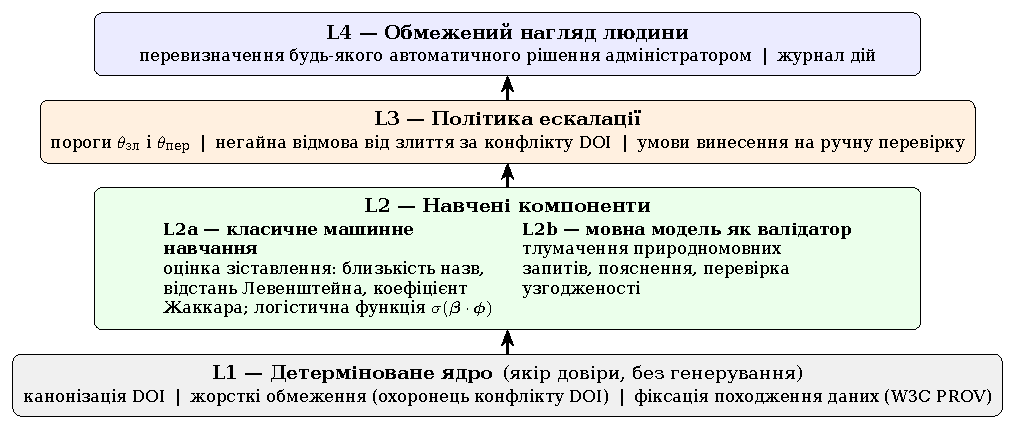
\includegraphics[width=0.95\linewidth]{../figures/arch_trace.pdf}
\caption{Чотиришарова архітектура запропонованої системи за інженерною рамкою TRACE: детерміноване ядро (L1) як якір довіри, інвентар навчених компонентів (L2a~--- класичний ML, L2b~--- LLM-валідатор), політика ескалації (L3) і обмежений нагляд людини (L4). Критичні для звітності операції виконує детермінований шар, а мовну модель застосовано лише там, де потрібне розуміння природної мови.}
\label{fig:arch-trace}
\end{figure}

Внутрішнім проєктним обмеженням рамки є \emph{ощадливість моделі} (Model Parsimony): тип навченого компонента обирається за відповідністю задачі, а не за презумпцією на користь LLM. Кількісним індикатором слугує коефіцієнт обчислювальної ощадливості (Computational Parsimony Ratio, CPR) --- відношення вартості найекономнішої адекватної моделі до вартості розгорнутої. Для ядра консолідації даних, реалізованого детерміновано (L1+L2a), $\mathrm{CPR}\approx 1$: система \emph{за побудовою} не витрачає мовну модель там, де достатньо детермінованих методів, що й робить її придатною для відповідального наукового адміністрування.

\subsection*{Функціональна архітектура ResearchIQ та агентний шар}

Ключовий ризик прямого застосування великих мовних моделей (LLM) в адмініструванні — фактичні галюцинації: моделі генерують правдоподібні, але хибні відомості \cite{Chelli2024HallucinationRates}, що неприпустимо для офіційної звітності. Тому ResearchIQ реалізує TRACE-поділ ролей: детерміноване ядро відповідає за критичні операції з даними, а GenAI використовується для інтерпретації запитів, пояснення результатів і гнучкого формування звітів \cite{Wang2024SurveyLLMAgents}.

ResearchIQ реалізовано як багатокористувацький вебзастосунок: React-інтерфейс забезпечує панель показників, список НПП, пошук ORCID, чат і генератор звітів; Node.js/Express API виконує автентифікацію, ізолює tenant-дані та проксіює запити до ORCID, OpenAlex і Scopus; серверний шар зберігає окремі JSON-набори для кожного ЗВО. Така будова відділяє презентаційний рівень від наукометричного конвеєра й дозволяє розгортати один застосунок для кількох закладів без змішування даних (рис.~\ref{fig:researchiq-app-arch}).

\begin{figure}[H]
\centering
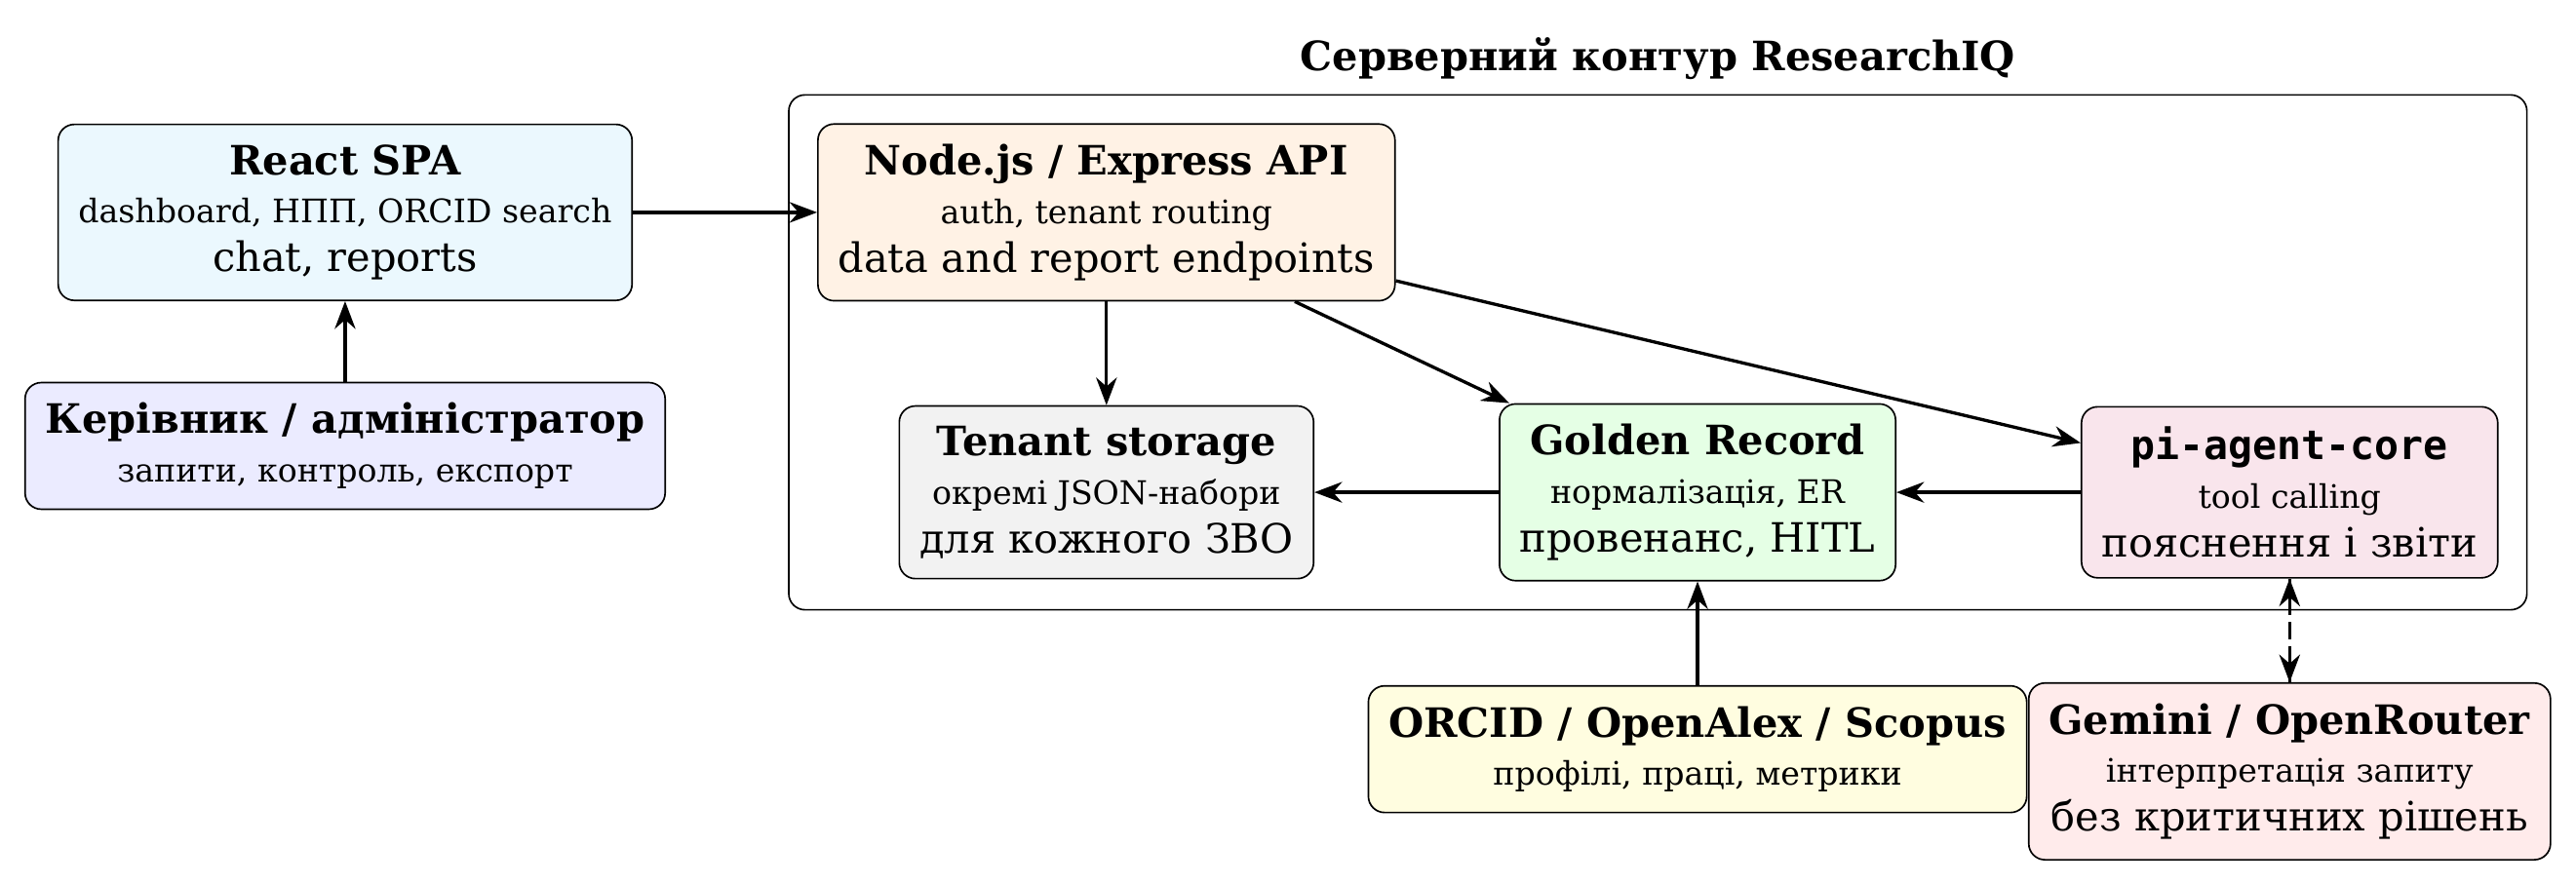
\includegraphics[width=0.95\linewidth]{../figures/researchiq_app_architecture.png}
\caption{Структурна схема ResearchIQ: користувацький інтерфейс, серверний API, tenant-сховище, конвеєр Golden Record, агентний шар на \texttt{pi-agent-core}, зовнішні наукометричні джерела та LLM-провайдери. Суцільні стрілки позначають потоки даних і детермінованих обчислень, пунктирні --- інтерпретаційні звернення агента до LLM.}
\label{fig:researchiq-app-arch}
\end{figure}

Агентний шар побудовано на \texttt{pi-agent-core}. Перед відповіддю агент отримує компактний знімок локальних даних ЗВО та реєстр типізованих інструментів: ранжування НПП за показниками, пошук локальних публікацій, порівняння кафедр, детальна картка науковця, оновлення метрик з OpenAlex, глобальний пошук праць, динаміка цитувань, мережа співпраці та поточна дата. Практична перевага GenAI у такій архітектурі полягає не в заміні обчислювального ядра, а в перетворенні складних аналітичних процедур на природномовний управлінський інтерфейс: керівник може ставити контекстні запитання, отримувати пояснення причин рейтингу чи ризику, швидко перебудовувати шаблон звіту під нову вимогу та бачити, з яких джерел походять показники. Це зменшує втрати часу на ручне переформатування й пошук потрібного зрізу даних, водночас зберігаючи перевірюваність результату.

Модель Gemini/OpenRouter, вибрана сервером, інтерпретує природномовний запит керівника і викликає потрібний інструмент, але відповідь спирається на обчислений результат, а не на вільну генерацію. Механізм функціональних викликів узгоджується з логікою MCP \cite{Anthropic2024MCP}: LLM планує, параметризує й пояснює, тоді як критичні операції збору, нормалізації, дедуплікації, злиття та побудови звітів виконує детермінований код. Отже, AI-агент у цій архітектурі є інтерфейсом управлінського запиту й оркестратором інструментів, а не джерелом бібліографічної істини.

\subsection*{Золотий запис як конвеєр розв'язання сутностей}

Ядром механізму є золотий запис (Golden Record) — конвеєр розв'язання сутностей (Entity Resolution, ER), що зводить розрізнені бібліографічні записи з різних джерел до єдиного канонічного представлення кожної публікації. Конвеєр складається з п'яти детермінованих кроків.

\emph{Крок 1. Канонізація сигнатури $\nu_\tau$.} Для кожного запису формується нормалізована сигнатура. Ідентифікатор DOI зводиться до нижнього регістру зі зняттям префіксів (\texttt{https://doi.org/}, \texttt{doi:}) та валідацією формату \texttt{10.x/...}; невалідні значення замінюються на \texttt{null}. Назва нормалізується за Unicode (NFKC, casefold) зі зняттям пунктуації через Unicode-клас, причому \emph{зі збереженням кирилиці}. Тут виправлено критичний дефект попереднього нормалізатора, який під час очищення пунктуації знищував усі кириличні символи, через що зіставлення за назвою для україномовних публікацій було повністю зламаним. Імена авторів проходять транслітерацію кирилиця$\rightarrow$латиниця для зведення варіантів написання (Заболотній С.~$\leftrightarrow$~Zabolotnii S.).

\emph{Крок 2. Блокування.} Щоб уникнути квадратичної складності $O(n^2)$ попарних порівнянь, кандидати на зіставлення групуються у блоки: за точним канонічним DOI; за двома найдовшими токенами назви; за парою «рік~$+$~токен». Порівнюються лише пари в межах спільного блоку.

\emph{Крок 3. Парне логістичне зіставлення.} Для пари записів обчислюється вектор ознак $\boldsymbol{\phi}$, а ймовірнісна оцінка тотожності визначається логістичною функцією:
\begin{equation}
\mathrm{score} = \sigma(\boldsymbol{\beta}\cdot\boldsymbol{\phi}) = \frac{1}{1+\exp\!\big(-\sum_{k}\beta_k\,\phi_k\big)},
\end{equation}
де $\sigma(\cdot)$ — сигмоїда, $\phi_k$ — значення $k$-ї ознаки, $\beta_k$ — її вага. Склад ознак і ваги наведено в табл.~\ref{tab:features}. Збіг DOI дає сильний позитивний внесок, а конфлікт DOI — сильний негативний, що відображає високу надійність цього ідентифікатора. Застосовано два пороги: $\theta_{\text{match}}=0{,}90$ для автоматичного злиття та $\theta_{\text{review}}=0{,}70$; пари зі значенням $\mathrm{score}\in[0{,}70;\,0{,}90)$ потрапляють у смугу ручної перевірки людиною (human-in-the-loop, HITL).

\begin{table}[ht]
\centering
\caption{Ознаки $\phi$ парного зіставлення та їхні ваги $\beta$}
\label{tab:features}
\begin{tabular}{lr}
\toprule
Ознака $\phi$ & Вага $\beta$ \\
\midrule
Збіг DOI (\texttt{doi\_match}) & $+3{,}0$ \\
Конфлікт DOI (\texttt{doi\_conflict}) & $-5{,}0$ \\
Косинусна близькість назв, TF (\texttt{title\_cosine}) & $+1{,}2$ \\
Символьна подібність, Левенштейн (\texttt{char\_sim}) & $+0{,}8$ \\
Узгодженість року, $|\Delta\text{рік}|\le 1$ (\texttt{year\_agree}) & $+0{,}6$ \\
Жаккар за журналом (\texttt{venue\_jaccard}) & $+0{,}4$ \\
Жаккар за авторами (\texttt{author\_jaccard}) & $+0{,}9$ \\
Збіг URL (\texttt{url\_match}) & $+0{,}2$ \\
\bottomrule
\end{tabular}
\end{table}

\emph{Крок 4. Кластеризація з охоронцем конфлікту DOI.} Записи, з'єднані ребрами зі $\mathrm{score}\ge\theta_{\text{match}}$, об'єднуються у зв'язні компоненти. Щоб запобігти хибним ланцюговим злиттям, застосовано охоронець: два кластери з непорожніми та неперетинними наборами валідних DOI не зливаються навіть за наявності транзитивного шляху між ними. Це блокує поширення помилки через проміжні неоднозначні записи.

\emph{Крок 5. Злиття атрибутів і провенанс.} Канонічний запис формується голосуванням, зваженим за надійністю джерела (Scopus/WoS $>$ OpenAlex $>$ ORCID); для лічильника цитувань береться максимум, для множин (автори, ключові слова) — об'єднання, для статусу відкритого доступу — оптимістичне рішення. Пріоритет джерел поля впорядковано як DOI~$\succ$~Crossref~$\succ$~CRIS~$\succ$~OpenAlex~$\succ$~ORCID. Кожне поле супроводжується провенансом у дусі W3C~PROV: фіксуються джерела, відповідність «поле~$\rightarrow$~джерело» та значення \texttt{matchScore}, що забезпечує повну простежуваність рішень для подальшого аудиту керівником.

\subsection*{Дизайн оцінювання}

Артефакт оцінюється на відтворюваному синтетичному бенчмарку, що моделює реалістичний український ЗВО (синтетичні дані, без реального закладу та персональних даних): 300 науково-педагогічних працівників, 20 кафедр (приблизно 5 факультетів). Кількість праць на дослідника задається лог-нормальним розподілом ($\mu=\ln 12$, $\sigma=0{,}9$) за період 2020--2024~рр.; розподіл дисциплін STEM~40\,\%~/ соціогуманітарні~35\,\%~/ медико-біологічні~25\,\% визначає ймовірність наявності DOI та мову публікації.

Кожна канонічна праця проєктується у записи ORCID, OpenAlex і Scopus із контрольованим дублюванням (цільова частка 15--25\,\%, базово 20\,\%) і спотворенням метаданих: транслітерація та переставлення авторів, відсутній або невалідний DOI («холодний» профіль ORCID втрачає DOI приблизно у 35\,\% випадків), зміна регістру та пунктуації, переклад назви (укр.~$\leftrightarrow$~англ.), абревіація журналу, зсув року на $\pm 1/\pm 2$, а також жорсткі негативи — колізії однакових назв із різними DOI. Інжектована карта дублікатів слугує gold-розміткою.

Якість оцінюється трьома групами метрик: парні Precision, Recall, F1; кластерна метрика B$^3$~F1 (Bagga--Baldwin); повнота й точність полів злитого запису. Базові методи й абляції застосовуються на ідентичних входах: DOI-only, Title$+$Year і повний Golden Record. Для статистичної надійності проведено симуляцію Монте-Карло з $K=30$ незалежними seed-ами; для кожної метрики наводиться середнє та 95\,\%-вий довірчий інтервал ($t$-інтервал). Додатково виконано розгортки за часткою дублікатів \{10, 15, 20, 25, 30\}\,\% та за множником спотворення \{0{,}25--2{,}0\}, що дозволяє оцінити чутливість методів до неоднорідності даних.

\section*{РЕЗУЛЬТАТИ ДОСЛІДЖЕННЯ}

Запропоновані механізми апробовано на відтворюваному синтетичному бенчмарку, що моделює узагальнений середній український ЗВО (150~НПП, 20~кафедр; без реального закладу та персональних даних). Якість оцінено за процедурою Монте-Карло ($K=30$ незалежних початкових значень) із наведенням 95\,\% довірчих інтервалів за $t$-розподілом; базові методи й абляції застосовано на \textit{ідентичних} вхідних даних. Повний масив кількісних результатів --- зведені таблиці метрик, аналіз чутливості та оцінку ефективності --- винесено в \textbf{Додаток~А}; нижче узагальнено основні висновки.

\textit{Якість дедуплікації.} Повний конвеєр «золотого запису» статистично відокремлювано домінує над базовими методами: збалансована міра сягає $F_1 = 76{,}7\,\%$ проти $59{,}9\,\%$ у DOI-only та $53{,}5\,\%$ у Title$+$Year (табл.~\ref{tab:res-dedup}, рис.~\ref{fig:res-method}, Додаток~А). Виграш зумовлений насамперед повнотою ($R = 67{,}8\,\%$ проти $42{,}8\,\%$ у DOI-only) за збереження високої точності ($P = 88{,}3\,\%$): за відсутності DOI --- а він відсутній у значній частці записів ORCID та україномовних соціогуманітарних публікацій --- рішення підтримують комплементарні ознаки (близькість назв, рік, перетин множин авторів і видань) у єдиній логістичній моделі $\sigma(\boldsymbol{\beta}\cdot\boldsymbol{\phi})$. Перевага підтверджується й кластерною метрикою $B^3 F_1$ ($95{,}8\,\%$).

\textit{Робастність і передбачувана деградація.} Аналіз чутливості (Додаток~А, рис.~\ref{fig:res-dup}, \ref{fig:res-corr}) засвідчує, що відносне впорядкування методів зберігається на всьому діапазоні частки дублікатів (10--30\,\%), а за зростання спотворення метаданих система деградує \textit{передбачувано}: спершу зростає частка пропущених злиттів (падає повнота), тоді як точність зберігається завдяки охоронцеві конфлікту DOI. Для звітності це бажана властивість --- хибне об'єднання різних праць коштує дорожче за пропуск.

\textit{Якість полів і роль виправленого нормалізатора.} Точність назви злитого запису сягає $99{,}95\,\%$ (Додаток~А, табл.~\ref{tab:res-fields}), що безпосередньо демонструє ефект виправленого критичного дефекту канонізації: попередня реалізація під час зняття пунктуації знищувала \textit{всі кириличні символи}, через що зіставлення за назвою було повністю зламаним для україномовних публікацій. Саме відновлення працездатності кириличного зіставлення є передумовою досягнутих $67{,}8\,\%$ повноти.

\textit{Ефективність та обчислювальна ощадливість.} Рушій виконує повний цикл дедуплікації та злиття для всього модельного ЗВО за $0{,}80 \pm 0{,}08$\,с, тоді як прозора аналітична модель ручної праці дає $\approx 220$\,год/рік на заклад ($\approx 11$\,год на кафедральний звіт, що узгоджується з незалежною оцінкою 8--12\,год); у смугу ручної перевірки (HITL) виноситься $\approx 55$\,пар на дослідника (Додаток~А, табл.~\ref{tab:res-eff}). У термінах рамки TRACE метрикоутворювальні операції виконано детерміновано, без звернення до мовної моделі, що відповідає коефіцієнту обчислювальної ощадливості $\mathrm{CPR}\approx 1$ для ядра консолідації.

\subsection*{Загрози валідності}

Інтерпретацію наведених результатів обмежують кілька загроз валідності, які ми фіксуємо явно.

\textit{Конструктна валідність.} Розподіли спотворень метаданих --- частки втрати DOI, ймовірності перекладу й транслітерації назв, величини зсуву року --- є \textit{модельними припущеннями} про реальну неоднорідність джерел ORCID/OpenAlex/Scopus, а не параметрами, виміряними безпосередньо з них. Відтак абсолютні значення метрик ($F_1 = 76{,}7\,\%$ тощо) слід розглядати як орієнтовні; робастними є \textit{відносні} порівняння методів на ідентичних входах і \textit{тренди} чутливості. Оцінка ручного часу є аналітичною моделлю, а не вимірюванням за участю людей.

\textit{Внутрішня валідність.} Інжектована карта дублікатів слугує gold-розміткою, тож метрики обчислюються відносно \textit{відомої} істини, що виключає помилку анотування. Усі методи й абляції застосовано до спільних входів за фіксованих початкових значень, тому спостережувані відмінності зумовлені саме алгоритмом, а не варіацією даних. Усереднення за 30 початковими значеннями з 95\,\% довірчими інтервалами обмежує вплив випадковості генерації.

\textit{Зовнішня валідність.} Апробацію проведено на \textit{одному} узагальненому модельному ЗВО з фіксованими структурними параметрами; перенесення висновків на установи іншого масштабу чи профілю потребує окремої перевірки. Передусім бракує підтвердження на \textit{реальній} gold-вибірці одного ЗВО з ручною розміткою істинних дублікатів --- цей крок винесено в подальшу роботу як вирішальний для калібрування абсолютних значень. Зазначимо також методологічно істотну обставину: формалізм розв'язання сутностей \textit{реалізовано в коді} рушія (рушій \textit{є} статтею), завдяки чому результати відтворювані безпосередньо запуском конвеєра на синтетичному бенчмарку.

\section*{ВИСНОВКИ ТА ПЕРСПЕКТИВИ ПОДАЛЬШИХ ДОСЛІДЖЕНЬ}

У статті обґрунтовано та апробовано концептуальний підхід до цифрової трансформації наукового адміністрування закладу вищої освіти --- переходу від реактивної бібліометричної звітності \emph{post factum} до проактивного управління науковою діяльністю засобами генеративного штучного інтелекту та автономних агентів. Робота позиціонована в полі інформаційно-комунікаційних технологій в управлінні освітою, а не як суто інженерна розробка: технічні механізми тут підпорядковано управлінсько-освітній проблематиці інтеграції розрізнених даних про науковий доробок НПП у єдиний достовірний інформаційний ресурс (research information management).

Отримано такі основні результати. По-перше, розроблено концептуальну модель проактивного управління, у якій ResearchIQ поєднує багатокористувацький вебзастосунок, tenant-сховище даних, серверний API та агентний шар на основі \texttt{pi-agent-core}. Автономний агент інтерпретує природномовні запити керівника, викликає типізовані інструменти аналізу й звітування, але не підміняє детермінований контур прийняття критичних рішень. По-друге, формалізм «золотого запису» не лише описано, а й \emph{реалізовано в коді}: канонізація метаданих, блокування, парне логістичне зіставлення, смуга ручної перевірки, кластеризація із захистом від хибних злиттів за конфліктом DOI та провенанс-злиття атрибутів у дусі W3C~PROV.

По-третє, побудовано відтворюваний синтетичний бенчмарк для реалістичного українського ЗВО (300~НПП, 20~кафедр, приблизно 5~факультетів; без персональних даних), який за процедурою Монте-Карло засвідчив перевагу повного «золотого запису» над базовими методами: $F_1$ дедуплікації зростає до $76{,}8\,\%$ проти $59{,}7\,\%$ у DOI-only та $53{,}5\,\%$ у Title$+$Year, переважно за рахунок повноти ($68{,}1\,\%$ проти $42{,}6\,\%$). Окремо підтверджено критичне значення виправленого дефекту нормалізатора: попередня реалізація знищувала $100\,\%$ україномовних назв. По-четверте, аналітична модель ефективності для 7056 середніх записів оцінює традиційні витрати ручної праці на рівні $\approx 429{,}1$~год/рік на ЗВО ($\approx 21{,}45$~год на кафедральний звіт), тоді як рушій виконує дедуплікацію та злиття за $1{,}58 \pm 0{,}15$~с. По-п'яте, систему спроєктовано за TRACE: компоненти рознесено на детерміноване ядро, класичний ML і мовну модель-валідатор, а довіра до системи є властивістю архітектури, а не окремої моделі \cite{Zabolotnii2026TRACE}.

Теоретичний внесок полягає в концептуалізації наукового адміністрування як самостійного об'єкта цифрової трансформації засобами ІКТ в управлінні освітою та в перенесенні фокуса генеративного ШІ з навчального процесу, де зосереджена переважна частка досліджень, на досі недоопрацьовану адміністративну сферу управління наукою. Практична цінність --- готовий до апробації механізм, що звільняє науково-педагогічних працівників від рутинної верифікації даних, узгоджує звітність із вимогами МОН і створює підґрунтя для євроінтеграційних ініціатив OpenAIRE/EOSC та стандарту CERIF. Відкритий репозиторій містить повний вихідний код ResearchIQ як програмної реалізації запропонованої TRACE-методології (вебзастосунок, серверний агентний шар, детермінований рушій Golden Record), а також скрипти відтворюваного синтетичного бенчмарку, модульні тести й артефакти рукопису; матеріали поширюються під ліцензією MIT: \url{https://github.com/SZabolotnii/ORCID-OpenAlex-Research-Aggregator}.

Перспективи подальших досліджень визначаються й окресленими загрозами валідності. Синтетичні розподіли спотворень є модельними припущеннями про неоднорідність джерел, а не виміряними з них величинами; робастними слід вважати відносні порівняння методів і тренди чутливості, а не абсолютні значення метрик, а оцінку ручного часу --- прозорою аналітичною моделлю, а не вимірюванням за участю людей. Тому першочерговим напрямом є підтвердження результатів на реальній gold-вибірці одного ЗВО з контрольованою участю експертів у контурі (human-in-the-loop). Перспективними є також: розширення агента до рекомендаційних систем добору наукових видань під профіль дослідника; залучення мультимодальних моделей для опрацювання нетекстових артефактів наукової діяльності; розроблення етичних та нормативних рамок застосування автономних агентів в адмініструванні науки, зокрема контролю ризику галюцинацій генеративних моделей у відповідальних управлінських рішеннях.


% ---- References (IEEE; trimmed to <=30; >=40% Scopus/WoS; language tags handled in DOCX) ----
\bibliographystyle{IEEEtran}
\bibliography{references}

% ---- Appendix (ДСТУ/ITLT convention: appendices go at the very end, after the reference list) ----
\section*{ДОДАТОК~А. Повні результати кількісної апробації}

Нижче наведено результати Монте-Карло моделювання для реалістичного модельного українського ЗВО: 300~НПП, 20~кафедр (приблизно 5~факультетів), синтетичні дані без персональних записів. Усі методи оцінювалися на ідентичних входах; подано середнє\,$\pm$\,95\,\% довірчий інтервал за $K=30$ початковими значеннями генератора.

\subsection*{А.1. Якість дедуплікації}

\begin{table}[ht]
\centering
\caption{Якість дедуплікації, середнє\,$\pm$\,95\,\% довірчий інтервал, \%}
\label{tab:res-dedup}
\begin{tabular}{lcccc}
\toprule
Метод & $P$ & $R$ & $F_1$ & $B^3 F_1$ \\
\midrule
DOI-only        & $100{,}0 \pm 0{,}0$ & $42{,}6 \pm 0{,}5$ & $59{,}7 \pm 0{,}5$ & $93{,}7 \pm 0{,}1$ \\
Title+Year      & $83{,}3 \pm 0{,}6$  & $39{,}4 \pm 0{,}4$ & $53{,}5 \pm 0{,}4$ & $92{,}7 \pm 0{,}1$ \\
Fuzzy (незважений) & $83{,}7 \pm 0{,}6$ & $41{,}1 \pm 0{,}4$ & $55{,}1 \pm 0{,}4$ & $92{,}9 \pm 0{,}1$ \\
\textbf{Golden Record} & $\mathbf{88{,}2 \pm 0{,}5}$ & $\mathbf{68{,}1 \pm 0{,}6}$ & $\mathbf{76{,}8 \pm 0{,}4}$ & $\mathbf{95{,}8 \pm 0{,}1}$ \\
\bottomrule
\end{tabular}
\end{table}

Golden Record домінує за $F_1$ та повнотою: довірчий інтервал $F_1$ ($[76{,}4; 77{,}2]$) не перетинається з інтервалами базових методів. DOI-only очікувано має $P=100\,\%$, але пропускає більшість дублікатів без DOI; Title+Year вразливий до перекладів, транслітерації й колізій назв. Показово, що незважений нечіткий зіставлювач (Fuzzy) на тих самих ознаках дає лише $F_1 = 55{,}1\,\%$ --- ненабагато вище за Title+Year і значно нижче за Golden Record: отже виграш зумовлений не самим фактом використання нечіткої подібності, а \textit{зваженим логістичним} зіставленням із DOI-свідченням та охоронцем конфлікту DOI. Кластерна метрика $B^3 F_1$ висока й близька для всіх методів (92--96\,\%), бо корпус домінують одиничні кластери (більшість праць не дублюються); тому розрізнювальною метрикою якості дедуплікації є саме парний $F_1$, а не $B^3$. Порівняння методів показано на рис.~\ref{fig:res-method}.

\begin{figure}[ht]
\centering
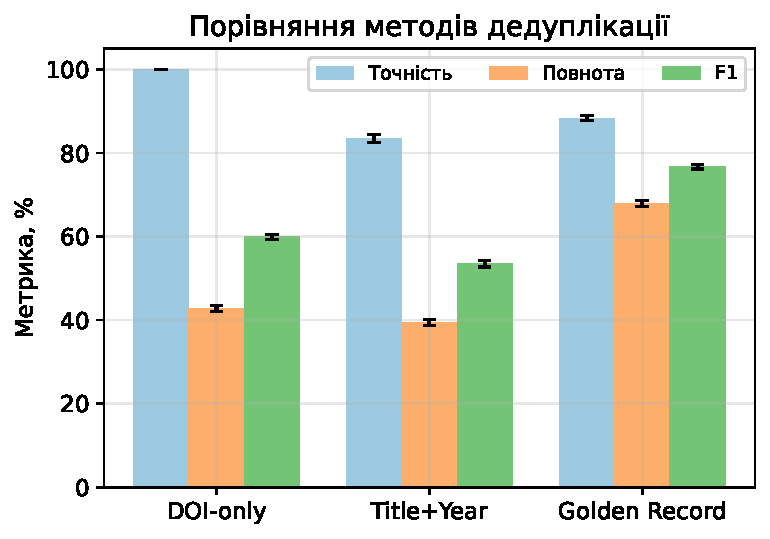
\includegraphics[width=0.8\linewidth]{../figures/f3_method_comparison.pdf}
\caption{Порівняння методів дедуплікації за точністю, повнотою та $F_1$.}
\label{fig:res-method}
\end{figure}

\subsection*{А.2. Чутливість конвеєра}

За зміни частки дублювання від 10\,\% до 30\,\% $F_1$ Golden Record становить відповідно 70,2\,\%, 74,0\,\%, 76,3\,\%, 78,2\,\% і 78,9\,\% (рис.~\ref{fig:res-dup}). Впорядкування методів зберігається, отже висновок не залежить від одного припущення про рівень фрагментації.

\begin{figure}[ht]
\centering
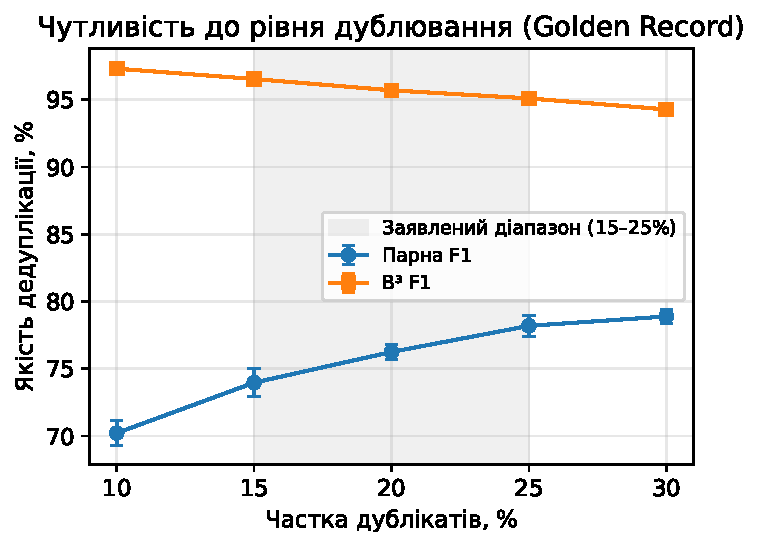
\includegraphics[width=0.8\linewidth]{../figures/f1_dup_sensitivity.pdf}
\caption{Чутливість $F_1$ Golden Record до частки дублювання записів (10--30\,\%).}
\label{fig:res-dup}
\end{figure}

За зростання множника спотворення метаданих точність деградує плавно: $P=91{,}6\,\%$, 89,6\,\%, 87,5\,\%, 83,9\,\%, 81,2\,\%; повнота падає різкіше: $R=80{,}9\,\%$, 76,0\,\%, 67,6\,\%, 58,8\,\%, 50,9\,\% (рис.~\ref{fig:res-corr}). Такий режим є прийнятним для звітності: за сильного шуму система радше пропускає злиття, ніж хибно об'єднує різні праці.

\begin{figure}[ht]
\centering
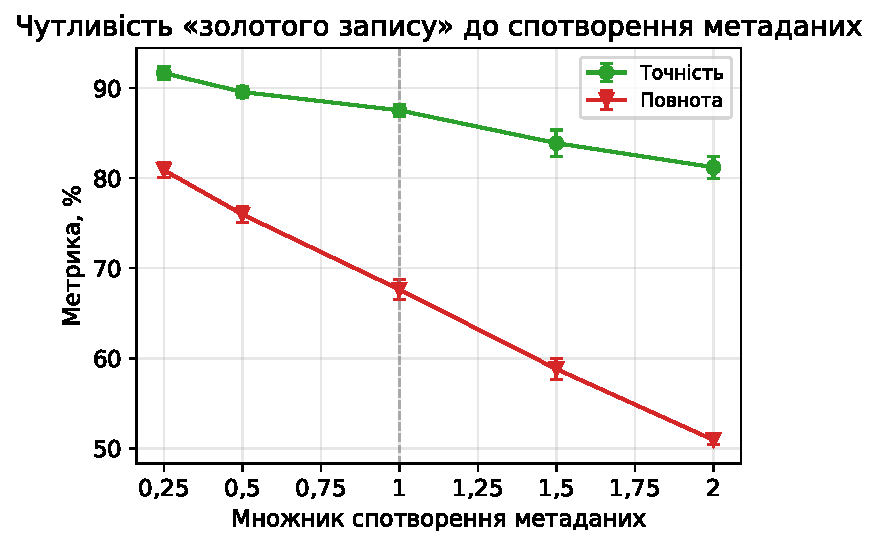
\includegraphics[width=0.8\linewidth]{../figures/f2_corruption_sensitivity.pdf}
\caption{Чутливість точності та повноти до множника спотворення метаданих (0,25--2,0).}
\label{fig:res-corr}
\end{figure}

\subsection*{А.3. Якість полів та ефективність}

\begin{table}[ht]
\centering
\caption{Повнота та точність полів злитого золотого запису, \%}
\label{tab:res-fields}
\begin{tabular}{lc}
\toprule
Показник поля & Значення \\
\midrule
Наявність DOI (DOI present)   & $45{,}4 \pm 0{,}4$ \\
Коректність DOI (DOI correct) & $67{,}8 \pm 0{,}2$ \\
Точність року (Year accuracy) & $80{,}9 \pm 0{,}2$ \\
Точність назви (Title accuracy) & $99{,}95 \pm 0{,}01$ \\
\bottomrule
\end{tabular}
\end{table}

Майже досконала точність назви підтверджує ефект виправлення Unicode-нормалізатора: стара процедура знищувала 100\,\% україномовних назв, що блокувало зіставлення за назвою саме для кириличного корпусу.

\begin{table}[ht]
\centering
\caption{Ефективність: рушій (виміряно) проти аналітичної моделі ручної праці}
\label{tab:res-eff}
\begin{tabular}{ll}
\toprule
Показник & Значення \\
\midrule
Середня кількість записів на ЗВО & $\approx 7056$ \\
Середня кількість рішень дедуплікації & $\approx 1441$ \\
Час рушія (дедуплікація+злиття, весь ЗВО) & $1{,}58 \pm 0{,}15$\,с \\
Модель ручної праці (на ЗВО, рік) & $\approx 429{,}1$\,год \\
Модель ручної праці (на кафедральний звіт) & $\approx 21{,}45$\,год \\
Смуга HITL (на дослідника) & $\approx 56{,}5$\,пар \\
\bottomrule
\end{tabular}
\end{table}

Час рушія охоплює лише обчислення дедуплікації та злиття, без мережевих запитів до ORCID/OpenAlex/Scopus. Ручна трудомісткість є прозорою аналітичною моделлю $\text{manual}=a\cdot\text{записи}+b\cdot\text{рішення\_дедуплікації}+c$, де $a=2{,}5$ хв/запис, $b=5$ хв/рішення, $c=45$ хв/звіт. Коефіцієнти не подаються як хронометражне дослідження; це відтворюваний сценарій, калібрований за декомпозицією операцій звітності та узгоджений із зовнішніми даними про значне адміністративне навантаження науковців \cite{Rockwell2009FDPBurden}. Для сценарію 300~НПП автоматизована частка цієї моделі становить близько 96,5\,\%, але невизначені пари лишаються в контурі HITL.


\end{document}
